% Figure 1: how the paper reads a prompt, and what sets a description's worth.
% Compile: latexmk -cd -pdf -interaction=nonstopmode -halt-on-error docs/paper/figs/overview.tex
% ESS values in (b) are copied from Table 2 (results/rq2-reliability/ess_map.csv,
% d = 16, a0 = 10, N = 1): 7.6, 116.5, 23.1. Prior shapes are sketches.
\documentclass[border=0pt]{standalone}
\usepackage[scaled=0.92]{helvet}
\usepackage{sansmath}
\usepackage{amsmath}
\usepackage{tikz}
\usetikzlibrary{arrows.meta, positioning, calc, decorations.pathreplacing}

\definecolor{orxblue}{HTML}{0072B2}
\definecolor{orxorange}{HTML}{E69F00}

\tikzset{
  orx/.style={font=\sffamily\sansmath\footnotesize, >={Stealth[round, length=4pt, width=3pt]},
    line width=0.5pt},
  tok/.style={draw=black!45, fill=white, rounded corners=1.5pt, minimum height=6mm,
    minimum width=10mm, inner sep=2pt},
  desc/.style={tok, draw=orxorange, fill=orxorange!14, line width=0.7pt},
  ex/.style={tok, draw=orxblue!70, fill=orxblue!8},
  brace/.style={decorate, decoration={brace, amplitude=3pt, raise=1.5mm}, draw=black!50},
  lbl/.style={font=\sffamily\sansmath\scriptsize, text=black!65, align=center},
  panel/.style={font=\sffamily\bfseries\footnotesize, anchor=north west, inner sep=0pt},
  note/.style={font=\sffamily\sansmath\scriptsize, anchor=west, align=left},
}

% One example = one square. #1 anchor coordinate, #2 whole examples, #3 fraction of the last.
\newcommand{\pitch}{0.66mm}
\newcommand{\sq}{0.46mm}
\newcommand{\tick}{2.4mm}
\newcommand{\exbar}[3]{%
  \foreach \i in {1,...,#2} {\fill[orxblue] ($(#1)+({(\i-1)*\pitch}, -\tick/2)$) rectangle +(\sq, \tick);}
  \fill[orxblue] ($(#1)+({#2*\pitch}, -\tick/2)$) rectangle +({#3*\sq}, \tick);
}

% A prior sketch on a 24 mm axis (w from -3 to 3), mean of the description at w = 1.2.
% #1 anchor (left end of the axis), #2 the description's density as a function of \x.
\newcommand{\prior}[2]{%
  \begin{scope}[shift={(#1)}, x=4mm, y=1mm]
    \draw[black!30, dashed, line width=0.4pt, domain=-3:3, samples=60, smooth]
      plot ({\x+3}, {3*exp(-\x*\x/2)});
    \fill[orxorange!25, domain=-3:3, samples=160, smooth]
      plot ({\x+3}, {#2}) -- (6,0) -- (0,0) -- cycle;
    \draw[orxorange, line width=0.7pt, domain=-3:3, samples=160, smooth] plot ({\x+3}, {#2});
    \draw[black!60] (0,0) -- (6,0);
    \draw[black!60] (4.2,0) -- (4.2,-0.8) node[below, lbl, inner sep=1pt] {$m$};
  \end{scope}
}

\begin{document}
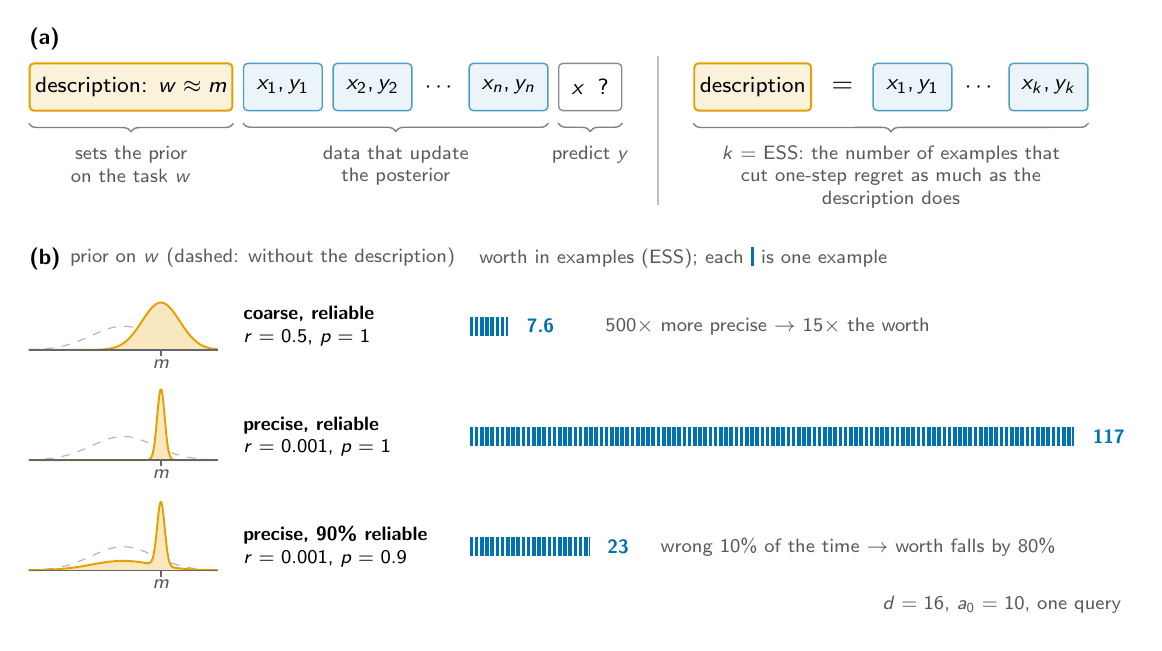
\begin{tikzpicture}[orx]

  % ---------- (a) the prompt as Bayesian inference, and the ESS ----------
  \node[panel] (pa) at (0,0) {(a)};

  \node[desc, anchor=north west] (d) at (0,-4.5mm) {description: $w \approx m$};
  \node[ex, right=1.2mm of d]  (e1) {$x_1, y_1$};
  \node[ex, right=1.2mm of e1] (e2) {$x_2, y_2$};
  \node[right=0.3mm of e2]     (ed) {$\cdots$};
  \node[ex, right=0.3mm of ed] (en) {$x_n, y_n$};
  \node[tok, right=1.2mm of en, minimum width=8mm] (q) {$x \;\; ?$};

  \draw[brace] (d.south east) -- node[below=9pt, lbl] {sets the prior\\on the task $w$} (d.south west);
  \draw[brace] (en.south east) -- node[below=9pt, lbl] {data that update\\the posterior} (e1.south west);
  \draw[brace] (q.south east) -- node[below=9pt, lbl] {predict $y$} (q.south west);

  % right half: the exchange rate
  \node[desc, right=9mm of q] (d2) {description};
  \node[right=1.2mm of d2, font=\sffamily\sansmath\normalsize] (eq) {$=$};
  \node[ex, right=1.2mm of eq] (k1) {$x_1, y_1$};
  \node[right=0.3mm of k1]     (kd) {$\cdots$};
  \node[ex, right=0.3mm of kd] (kk) {$x_k, y_k$};
  \draw[brace] (kk.south east) -- node[below=9pt, lbl]
    {$k$ = ESS: the number of examples that\\cut one-step regret as much as the\\description does}
    ($(d2.south west)$);
  \draw[black!25] ($(q.east)!0.5!(d2.west) + (0,4mm)$) -- ++(0,-19mm);

  % ---------- (b) what sets the worth ----------
  \node[panel] (pb) at (0,-28mm) {(b)};
  \node[lbl, anchor=west] at (4mm,-28mm-1.3mm) {prior on $w$ (dashed: without the description)};
  \node[lbl, anchor=west] at (56mm,-28mm-1.3mm) {worth in examples (ESS); each \tikz[baseline=0.3mm]\fill[orxblue] (0,0) rectangle (\sq,\tick); is one example};

  % rows: prior sketch at x = 0..24 mm, labels at 26 mm, bars from 56 mm
  \coordinate (r1) at (0,-41mm);
  \coordinate (r2) at (0,-55mm);
  \coordinate (r3) at (0,-69mm);

  \prior{r1}{6*exp(-(\x-1.2)*(\x-1.2)/(2*0.36))}
  \prior{r2}{9*exp(-(\x-1.2)*(\x-1.2)/(2*0.0144))}
  \prior{r3}{8.1*exp(-(\x-1.2)*(\x-1.2)/(2*0.0144)) + 1.2*exp(-\x*\x/2)}

  \node[note] at ($(r1)+(26mm,3mm)$) {\textbf{coarse, reliable}\\$r = 0.5$, $p = 1$};
  \node[note] at ($(r2)+(26mm,3mm)$) {\textbf{precise, reliable}\\$r = 0.001$, $p = 1$};
  \node[note] at ($(r3)+(26mm,3mm)$) {\textbf{precise, 90\% reliable}\\$r = 0.001$, $p = 0.9$};

  \coordinate (b1) at ($(r1)+(56mm,3mm)$);
  \coordinate (b2) at ($(r2)+(56mm,3mm)$);
  \coordinate (b3) at ($(r3)+(56mm,3mm)$);
  \exbar{b1}{7}{0.6}
  \exbar{b2}{116}{0.5}
  \exbar{b3}{23}{0.1}
  \node[note, text=orxblue] at ($(b1)+(7.6*\pitch+1mm,0)$) {\textbf{7.6}};
  \node[note, text=orxblue] at ($(b2)+(116.5*\pitch+1mm,0)$) {\textbf{117}};
  \node[note, text=orxblue] at ($(b3)+(23.1*\pitch+1mm,0)$) {\textbf{23}};

  \node[note, text=black!65] at ($(b1)+(16mm,0)$) {500$\times$ more precise $\rightarrow$ 15$\times$ the worth};
  \node[note, text=black!65] at ($(b3)+(23mm,0)$) {wrong 10\% of the time $\rightarrow$ worth falls by 80\%};
  \node[lbl, anchor=north east] at ($(b3)+(84mm,-5mm)$) {$d = 16$, $a_0 = 10$, one query};

\end{tikzpicture}
\end{document}
